\chapter{Anwendung des Frameworks auf jadice flow}
\label{chap:anwendung}

In diesem Kapitel wird ein Architektur-Refactoring am Produkt \emph{jadice flow} geplant und in theoretischer Ebene durchgeführt.
Dazu werden \acrfull{mmf} und \acrfull{arh} benutzt, welche den Prozess sowie auch dieses Kapitel in drei Phasen unterteilen.
Eine genauere Beschreibung des Frameworks ist in \cref{sec:mmf} zu finden, sehr abstrahiert und vereinfacht bestehen die Phasen aus folgenden Aktivitäten:
\begin{itemize}
	\item In \cref{sec:durchführung-phase1} wird die Durchführung der ersten Phase in Form eines Architekturreviews mit den wichtigsten Stakeholdern beschreiben.
	\item Im Rahmen der zweiten Phase wird in \cref{sec:durchführung-phase2} nach adäquaten Migrationsstrategien gesucht.
	\item In \cref{sec:durchführung-phase3} wird in der dritten Phase nach profitablen Patterns und Best Practices gesucht.
\end{itemize}

\section{Phase 1 - Systemverständnis}
\label{sec:durchführung-phase1}

Das Ziel dieser Phase ist ein Verständnis des Systems aufzubauen.
Dieses Verständnis ist wichtig für spätere Entscheidungen.

\subsection{Qualitätsattribute}

Im ersten Schritt dieser ersten Phase werden die gewünschten \glspl{qa} des Systems gesammelt.
In dieser Phase wurde in einer Fokusgruppe ein Architekturreview nach \Citet{SVAHNBERG20071893} wie in \cref{sec:methodik-architekturreview} beschrieben durchgeführt.
Teil dieser Gruppe waren vier Softwareentwickler beziehungsweise -Architekten, der \acrlong{po} und der Autor selbst in der Rolle des Moderators.
Durch die ebenfalls in \cref{sec:methodik-architekturreview} beschriebenen Veränderungen an der Methodik von \Citet{SVAHNBERG20071893} wurde auch der geplante Zeitrahmen dieser Fokusgruppe auf lediglich 2 Stunden reduziert. Das liegt vor allem daran, dass die letzten Phasen nicht nötig waren, aber auch daran, dass alle Teilnehmer bereits vertraut mit dem Produkt und der Architektur und Funktionsweise des Systems waren.
Demnach konnte nach einer kurzen Einleitung in die verwendete Methodik sofort mit Schritt 2, dem Ordnen der \glspl{qa} nach Wichtigkeit gestartet werden.

Dafür sollte jeder Teilnehmer seine Einschätzung darüber, welche die wichtigsten drei Sub-\glspl{qa} sind, per Nachricht abgeben.
Die daraus resultierende Anzahl von Stimmen pro Sub-\gls{qa} ist in \cref{tab:phase1-qas-priority} zu sehen. 
\begin{table}
  \centering
  \begin{tabular}{m{2.6cm} m{3.2cm} m{1.3cm} m{1.3cm}}
    \toprule
    \textbf{\gls{qa}} & \textbf{Sub-\gls{qa}} & \textbf{Anzahl Stimmen} & \textbf{Priorität} \\ \midrule
    Scalability & & 4 & 1\\ \hline

    \multirow{8}{=}[-0.1cm]{Maintainability} & Modularity & 4 & 2 \\
    & Monitorability & 2 & \\
    & Modifiabiltiy & 1 &  \\
    & Reusability & 1 &  \\
    & Testability & 1 &  \\
    & Analysability & 1 &  \\
    & Manageability & 1 &  \\
    & Understandability & 1 &  \\ \hline

    \multirow{2}{=}[-0.05cm]{Performance} & Time Behavior & 2 & 3 \\
    & Resource Utilization & 1 &  \\ \hline

   \multirow{5}{=}[-0.1cm]{Portability} & Deployability & 2 & 4 \\
   & Installability & 1 &  \\
   & Adaptability & 1 &  \\
   & Replaceability & 1 &  \\
   & Agility & 1 &  \\ \hline

    \multirow{3}{=}[-0cm]{Reliability} & Fault Tolerance & 1 & 5 \\
    & Recoverability & 1 & 6 \\
    & Availability & 1 &  \\ \hline

    Security & Confidentiality & 1 &  \\
    \bottomrule
  \end{tabular}
  \caption[Priorisierung der (Sub-) QAs durch Umfrage im Architekturreview]{
    Priorisierung der (Sub-) QAs durch Umfrage im Architekturreview in Phase 1 der Migration.
  }
  \label{tab:phase1-qas-priority}
\end{table}

Dabei ist auffällig, dass die Summe aller Stimmen 29 beträgt, obwohl bei fünf Teilnehmern der Umfrage mit jeweils drei Stimmen insgesamt nur 15 Stimmen zu erwarten wären.
Die Differenz wird damit begründet, dass nicht alle Teilnehmer der Umfrage sich auf Sub-\glspl{qa} beschränkt haben, sondern auch die \glspl{qa} \emph{Performance}, \emph{Reliability}, \emph{Maintainability} und \emph{Portability} genannt wurden.
Auch wenn das nicht so vorgesehen war, wurde davon abgesehen, die Teilnehmer darauf hinzuweisen und es zu korrigieren, da die Ergebnisse nicht direkt zur Priorisierung der Attribute führen müssen.
Stattdessen wurden die Umfrageergebnisse und als vage Basis für eine freiere Diskussion um die Priorisierung benutzt, deren Ergebnis die schlussendliche Platzierung der wichtigsten sechs Sub-\glspl{qa} war, welche ebenfalls in \cref{tab:phase1-qas-priority} zu sehen ist.
Diese sind:
\begin{enumerate}
	\item \emph{Scalability}
	\item \emph{Modularity}
	\item \emph{Time Behavior}
	\item \emph{Deployability}
	\item \emph{Fault Tolerance}
	\item \emph{Recoverability}
\end{enumerate}
Die genaue Anzahl der wichtigsten (Sub-)Attribute war dabei nicht vorgeschrieben, sondern wurde ebenfalls von der Gruppe diskutiert und gemeinsam auf sechs festgelegt.

Im nächsten Schritt war die Aufgabe, für jedes dieser (Sub-) \glspl{qa} zwei Szenarien zu definieren, die das Attribut gut und auf verschiedene Arten beschreiben.
Dafür wurde keine spezielle Methodik angewandt, sondern in freier Diskussion der gesamten Gruppe von verschiedenen Teilnehmern der Reihe nach für die Attribute Szenarien vorgeschlagen und anschließend überarbeitet oder teilweise auch abgewiesen.
Wie in den resultierenden Szenarien in \cref{fig:scenarios} zu sehen ist, hat jedes (Sub-)Attribut zwei Szenarien, abgesehen von den letzten zwei.
Dafür gibt es zwei Gründe.
Erstens wurden für diese Subattribute nicht mehrere Szenarien gefunden, die sich ausreichend stark unterschieden hätten.
Ebenfalls wurde in dem Fall ein Szenario als ausreichend empfunden, da \emph{Reliability} das einzige \gls{qa} ist, für das mehrere Subattribute eingeschlossen wurden, zumal es das am geringsten priorisierte Attribut war.

Um zusätzliche eine Priorisierung der Szenarien vornehmen zu können, sieht der \gls{arh} jeweils eine dreistufige Bewertung der Szenarien hinsichtlich ihrer Wichtigkeit und ihrer technischen Schwierigkeit vor.
Diese wurde im nächsten Schritt vorgenommen.
Wieder wurde dabei die Methodik der offenen Diskussion verwendet.
Dabei wurden die Szenarien der Reihe nach TODO.



\begin{landscape}
	\begin{figure}
		\centering
		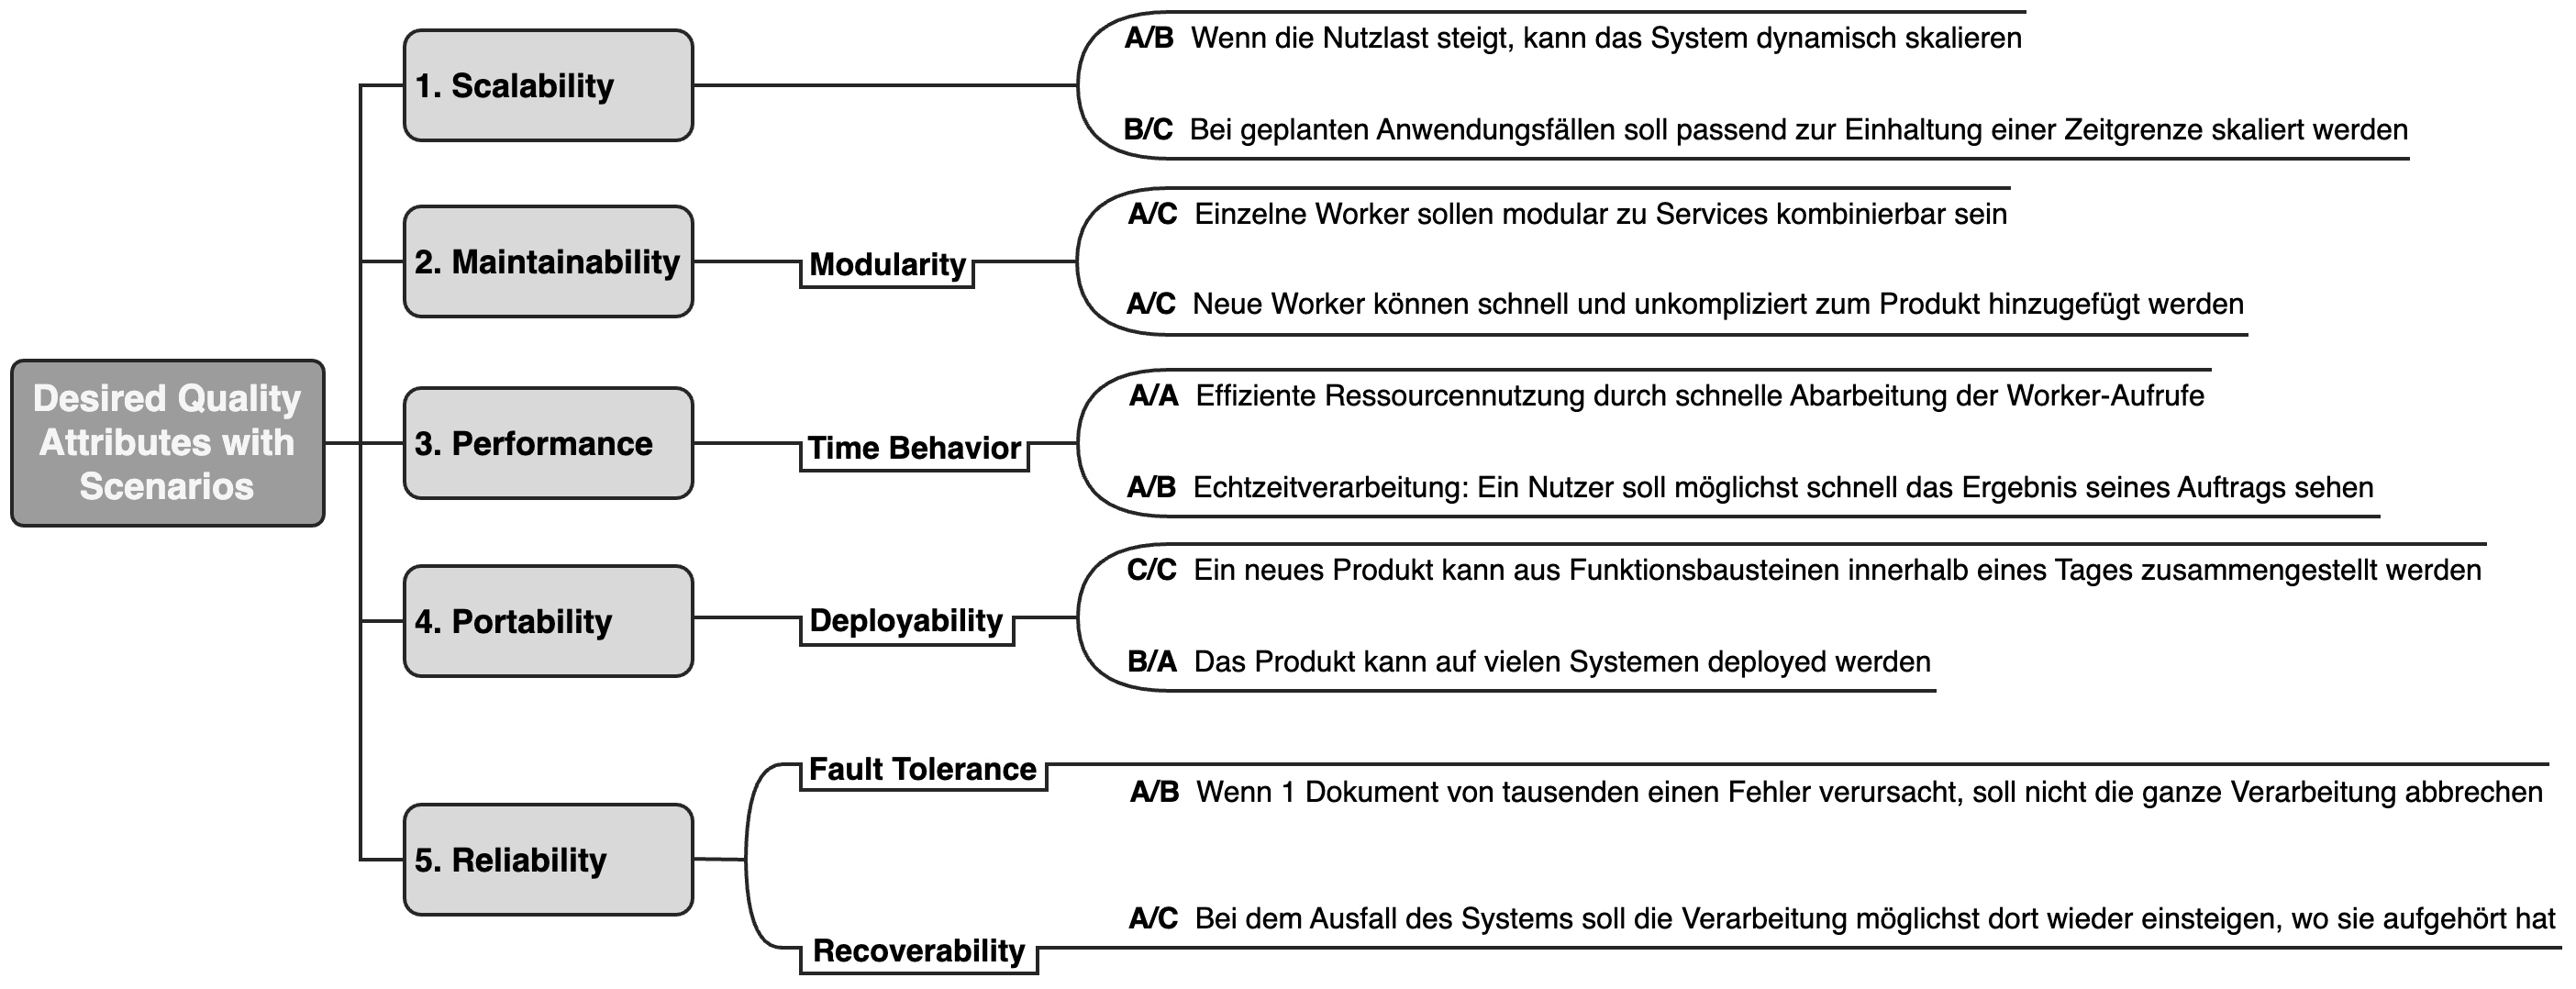
\includegraphics[width=1.5\textwidth]{scenarios.drawio}
		\caption[Utility Tree mit im Architekturreview ermittelten Qualitätsanforderungen und Szenarien]{
			Der Utility Tree mit Szenarien, die aus dem in Phase 1 durchgeführten Architekturreview resultieren.
			Von links nach rechts enthält der Baum folgende Elementarten: [1] Wurzel (ohne Bedeutung), [2] \gls{qa}, [3] Subattribut, [4] Beurteilung des Szenarios hinsichtlich Wichtigkeit und technischer Schwierigkeit, [5] Szenariobeschreibung.
		}
		\label{fig:scenarios}
	\end{figure}
\end{landscape}

Wie man in diesem Utility Tree sehen kann, sind die Szenarien nur mit jeweils einem \gls{qa} beziehungsweise Subattribut assoziiert.
Da realistischer Weise die meisten Szenarien allerdings mehrere \glspl{qa} beinhalten, wurden an einem zweiten Termin die Szenarien erneut betrachtet und diskutiert, welche weiteren \glspl{qa} sinnvoll hinzugefügt werden sollten.
Die resultierenden Assoziationen sind in der \cref{tab:scenarios} zu sehen.

\begin{table}[!h]
  \centering
  \begin{tabular}{ m{2,3cm} m{6cm} m{0.7cm} m{2,5cm} p{0.7cm} }
    \toprule
    \textbf{Name} & \textbf{Beschreibung} & \textbf{W/S} & \textbf{\glspl{qa}} & \textbf{MS} \\
    \midrule
    Dynamische Ska\-lier\-bar\-keit & Wenn die Nutzlast steigt, kann das Sys\-tem dynamisch skalieren & A/B & Scalability, Re\-source Uti\-li\-za\-tion, Adaptability, Execution Cost & \advantage \\ \hline
    Statische Ska\-lier\-bar\-keit & Bei geplanten Anwendungsfällen soll passend zur Einhaltung einer Zeitgrenze skaliert werden & B/C & Scalability, Resource Utilization, Time Behavior & \advantage \\  \hline
    Jobtemplates& Einzelne Worker sollen modular zu Services kombinierbar sein & A/C & Modularity, Reusability & - \\ \hline
    Neue Worker& Neue Worker können schnell und un\-kom\-pliziert zum Produkt hinzugefügt werden & A/C & Modularity, Reusability & \advantage  \\ \hline
    Schnelle Ab\-ar\-bei\-tung & Effiziente Ressourcennutzung durch schnelle Abarbeitung der Worker-Auf\-rufe  & A/A & Time Behavior, Resource Uti\-li\-za\-tion & \disadvantage \\ \hline
    \glqq Echtzeit\grqq{}-Verarbeitung & Ein Nutzer soll möglichst schnell das Ergebnis seines Auftrags sehen & A/B & Time Behavior & \disadvantage \\ \hline
    Einfaches De\-ploy\-ment & Ein neues Produkt kann aus Funk\-tions\-bausteinen innerhalb eines Tages zusammengestellt werden &C/C & Deployability, Modularity, Agility & \disadvantage \\ \hline
    Platform-unabhängigkeit& Das Produkt kann auf vielen Systemen deployed werden & B/A & Deployability, Installability & \advantage \\ \hline
    Fehlerto\-leranz Massen\-ver\-ar\-beitung & Wenn 1 Dokument von tausenden einen Fehler verursacht, soll nicht die ganze Verarbeitung abbrechen & A/B & Fault-Tolerance &\advantage \\ \hline
    Erholen nach Sys\-tem\-ausfall & Bei dem Ausfall des Systems soll die Verarbeitung möglichst dort wieder einsteigen, wo sie aufgehört hat & A/C & Recoverability & - \\
    \bottomrule
  \end{tabular}
  \caption[Im Architekturreview ermittelte Qualitätsanforderungen und Szenarien]{
    Szenarien, die aus dem in Phase 1 durchgeführten Architekturreview resultieren.
    \emph{W/S} gibt die Wichtigkeit/Schwierigkeit der Szenarien in drei Stufen an (A steht für sehr wichtig und sehr schwierig).
    \emph{\glspl{qa}} gibt die Assoziation der Szenarien zu bestimmten \acrfullpl{qa} an; zuerst genannte sind primäre \glspl{qa}, folgende sekundäre \glspl{qa}.
    \emph{MS} gibt die Einschätzung darüber an, ob das jeweilige Szenario von einer Microservices-Architektur profitiert.
  }
  \label{tab:scenarios}
\end{table}


Abschließend kann zu dieser Phase gesagt werden, dass sie größtenteils wie geplant durchgeführt werden konnte.
An einigen Stellen sind die verschiedene Schritte etwas verschmolzen oder es wurde kurz zu vorherigen Schritten zurückgesprungen.
Nicht alle Teilnehmer haben sich gleich stark beteiligt, doch vermutlich TODO

\subsection{Architekturbewertung}

Zusätzlich zum Erfassen der wichtigsten Szenarien und \glspl{qa} hatte die Fokusgruppe als sekundäres Ziel, die Wahl der Architektur für \emph{jadice flow} zu bewerten. 
Dies Entspricht dem vierten Schritt \emph{Assessment} der ersten Phase des \gls{arh}.
Da dieser im Werkzeug allerdings noch nicht implementiert ist, wurde der Schritt manuell durchgeführt.
Im Gegensatz zu vorherigen Schritten der ersten Phase ist dieser nicht relevant für die nächsten Phasen, weshalb es kein Problem ist, den \gls{arh} dabei nicht zu verwenden.
Im Rahmen dieses Schritts wurde diskutiert, ob eine Microservices-Architektur für jedes spezifische Szenario einzeln von Vorteil ist (gegenüber einer monolithischen Architektur), wobei sich auf lediglich drei Stufen festgelegt wurde:
\begin{itemize}
	\item \advantage\hspace*{0.1cm}: Dieses Szenario profitiert wesentlich mehr von einer \gls{msa} als von einer monolithischen Architektur.
	\item \disadvantage\hspace*{0.1cm}: Dieses Szenario profitiert wesentlich mehr von einer monolithischen Architektur als von einer \gls{msa}.
	\item \hspace*{0.27cm}-\hspace*{0.27cm}: Dieses Szenario profitiert in verschiedenen Punkten sowohl von einer \gls{msa} als auch von einer monolithischen Architektur, wobei sich beide Seiten ungefähr gleichen.
\end{itemize}
Bei Szenarios wie beispielsweise den des \emph{Scalability} Attributs war es nicht schwer, Konsens zu finden, da die Möglichkeit der Skalierung auf Service-Ebene einer der größten Vorteile von \glspl{msa} gegenüber Monolithen ist.
Doch in anderen Fällen war es schwieriger abzuwägen, ob die Vorteile einer \gls{msa} oder die eines Monolithen überwiegen.
Schlussendlich konnte jedoch in Form von offener  Diskussion für jedes Szenario einstimmig geklärt werden, welche der drei Optionen gewählt werden sollte, sodass keine Abstimmungen nötig waren.

Das Ergebnis dieser Einschätzungen ist ebenfalls in \cref{tab:scenarios} zu sehen.
Insgesamt in fünf Fällen wurde eine Microservices-Architektur als profitabel und nur in drei Fällen als unvorteilhaft eingeschätzt. 
Außerdem ist anzumerken, dass die Szenarien in der Tabelle nach der Wichtigkeit der primären \glspl{qa} sortiert ist und die obersten zwei Szenarien der hauptsächliche Treiber für die Migration zu einer Microservices-Architektur waren.
Durch die Überlegenheit der \gls{msa}-Favorisierungen und dass diese verstärkt bei den wichtigsten \glspl{qa} vorliegen kann diese Metrik die Entscheidung der Migration zu einer \gls{msa} bestätigen.

\section{Phase 2 - Strategieplanung}
\label{sec:durchführung-phase2}

In dieser Phase werden die Ergebnisse der Phase 1 in Form von \glspl{qa} beziehungsweise Szenarien genutzt, um eine passende Migrationsstrategie zu finden.
Dazu wurden die in \cref{tab:scenarios} dargestellten Szenarien bereits in den \gls{arh} eingegeben.
Zusätzlich werden in dieser Phase Filterkriterien definiert.
Mit deren Hilfe wird dann schlussendlich eine Liste von Migrationsstrategien vorgeschlagen, welche folgend analysiert wird.

\subsection{Filterselektion}
Damit bei der Suche nach Migrationsmethoden möglichst gut zum Zielsystem und den Vorstellungen der Architekten passende Ergebnisse vorgeschlagen werden, bietet der \gls{arh} neben der Konfiguration der Szenarien noch eine weitere Art, die Ergebnisse zu filtern und ordnen: Die Filter, die in diesem Abschnitt konfiguriert werden.
Dabei kann für jede der Eigenschaften aus \cref{tab:phase2-filter} eine dieser drei Präferenzen angegeben werden:
\begin{itemize}
	\item \textbf{Include:} Methoden, die die jeweilige Eigenschaft haben, werden höher platziert.
	\item \textbf{Neutral:} Ob Methoden die jeweilige Eigenschaft haben, wirkt sich nicht auf ihre Platzierung aus.
	\item \textbf{Exclude:} Methoden, die die jeweilige Eigenschaft nicht haben, werden höher platziert.
\end{itemize}


Für die Wahl der Filter für das Refactoring von \emph{jadice flow} haben \gls{po} und der Autor alle Filter betrachtet und die wichtigsten relevanten ausgewählt.
Diese sind \cref{tab:phase2-filter} farblich markiert.
Bewusst stammen die meisten gewählten Filter aus der Kategorie \emph{System Properties} gewählt. da diese als am ausschlaggebendsten für das System 
Der Grund dafür ist, dass bereits ohne Filtereinstellung das wichtigste 

Um bestmögliche Ergebnisse zu erhalten und dabei eine breite Abdeckung zu erhalten, wird das Suchverfahren mehrfach mit verschiedenen Filtereinstellungen wiederholt.

\begin{table}
  \centering
  \begin{tabular}{m{2cm} m{2cm} m{9cm}}
    \toprule
    \textbf{Kategorie} & \textbf{Subkategorie} & \textbf{Eigenschaften} \\
    \midrule
    Quality Preferences & System Properties & Autonomy, Cohesion, Complexity, Coupling, Granularity, Isolation, Technology Heterogenity \\ \hline
    \multirow{4}{=}[-1cm]{Input Preferences} & Domain Artifacts &  Documentation, Human expertise, Ontology, Version Control System \\ \cline{2-3}
    & Runtime artifacts & Log traces, User-Application interactions \\ \cline{2-3}
    & Model artifacts & Activity diagram, Business process model, Class diagram, Custom model, Data flow diagram, Entity model, State machine diagram, Use case model \\ \cline{2-3}
    & Executables & API / Interface, Database file, Source code (Java), Source code (No specification), Source code (Python), Test cases \\ \hline
    \multirow{6}{=}[-1.9cm]{Process Preferences} & Directions & Bottom-up, Mixed, Top-down \\ \cline{2-3}
    & Levels of automation & Automatic, Manual, Semi-automatic \\ \cline{2-3}
    & Analysis types & Dynamic, Historic, Lexical, Static \\ \cline{2-3}
    & Techniques & Clustering, Custom heuristics, Data-flow driven, Domain-Driven Design, Execution-trace modeling, General guidelines, Genetic algorithm, Graph-based, Machine Learning, Multi-Tenancy, Performance modeling, Scenario analysis, Wrapping / Black Box \\ \cline{2-3}
    & Process Strategy & Continuous Evolution, Extension, Greenfield, Refactor, Rewrite / Rebuild, Strangler \\ \cline{2-3}
    & Atomar Unit & Business Capability, Class, Entity, Function, Functionality, Interface, Other \\ \hline
    Output Preferences & Representation & Guideline / Workflow, List of services, Source code, Splitting recommendations, Visualization \\ \hline
    \multirow{4}{=}[-1cm]{Usability Preferences} &Validation methods & Case study, Experiment, Industry, No validation \\ \cline{2-3}
    & Accuracy of \gls{sia} & High, Medium, Low, Not available \\ \cline{2-3}
    & Tool supports &  No tool support \\ \cline{2-3}
    & Tool types & Database, Decomposition, Dynamic Analysis, Java, Open Source, Other, Reverse Engineering, Static Analysis, Visualization \\
    \bottomrule
  \end{tabular}
  \caption[Mögliche Filter des \gls{arh} in Phase 2]{
    Mögliche Filter des \gls{arh} in Phase 2.
  }
  \label{tab:phase2-filter}
\end{table}





Die Qualität dieser Filterfunktion soll ebenfalls in dieser Arbeit evaluiert werden, weshalb folgend in \cref{sec:phase2-ergebnisdurchsicht} die Ergebnisse verschiedener Filter betrachtet und verglichen werden.
Dafür wurden die Filter für das Refactoring von \emph{jadice flow} wie folgt gewählt.
Das Vorgehen ist in \cref{feldnotiz:1} dokumentiert.

\subsection{Suchergebnisbetrachtung}
\label{sec:phase2-ergebnisdurchsicht}

Die Filter, die im vorherigen Abschnitt gewählt wurden, werden in diesem Abschnitt angewendet, um jeweils geordnete Listen von Ergebnissen zu erhalten.
In Tabelle TODO werden

\begin{table}[!ht]
	\centering
	\begin{tabular}{l c c c}
		\toprule
    \textbf{Publikation} & \multicolumn{3}{c}{\textbf{Matches}} \\
     & \textbf{Insgesamt} & \textbf{\gls{qa}} & \textbf{\gls{sp}} \\ \midrule
    \multicolumn{4}{c}{\textbf{Alle Filter (15)}} \\ \midrule
    \Citet{arh-result-no-filter-1} & 15/32 & 11/17 & 0/5 \\ \hline
    \Citet{arh-result-no-filter-3} & 13/32 & 7/17  & 1/5  \\ \hline
    \Citet{arh-result-no-filter-2} & 12/32 & 7/17  & 2/5  \\ \hline
    \Citet{arh-result-no-filter-4} & 11/32 & 7/17  & 0/5  \\ \hline
    \Citet{arh-result-no-filter-5} & 11/32 & 7/17  & 0/5  \\ \midrule
		\multicolumn{4}{c}{\textbf{Wichtigste Filter (9)}} \\ \midrule
		\Citet{arh-result-no-filter-1}        & 14/26 & 11/17 & 0/3 \\ \hline
		\Citet{arh-result-no-filter-3}        & 13/26 & 7/17  & 1/3  \\ \hline
		\Citet{arh-result-no-filter-2}        & 11/26 & 7/17  & 1/3  \\ \hline
		\Citet{arh-result-important-filter-4} & 10/26 & 6/17  & 1/3  \\ \hline
    \Citet{arh-result-no-filter-4}        & 10/26 & 7/17  & 0/3  \\ \hline
    \textbf{\Citet{arh-result-no-filter-5}}        & 10/26 & 7/17  & 0/3  \\ \hline
    \textbf{\Citet{arh-result-important-filter-7}}        & 10/26 & 5/17  & 1/3  \\ \midrule
    \multicolumn{4}{c}{\textbf{Keine Filter (Nur \glspl{qa})}} \\ \midrule
    \Citet{arh-result-no-filter-1} & 11/17 & 11/17 & - \\ \hline
    \Citet{arh-result-no-filter-2} & 7/17  & 7/17  & - \\ \hline
    \Citet{arh-result-no-filter-3} & 7/17  & 7/17  & - \\ \hline
    \Citet{arh-result-no-filter-4} & 7/17  & 7/17  & - \\ \hline
    \Citet{arh-result-no-filter-5} & 7/17  & 7/17  & - \\ \bottomrule
	\end{tabular}
	\caption[Surchergebnisse des ARH von Migrationsverfahren mit verschiedenen Filtern]{
		Ergebnisse der Suche mit ARH nach Migrationsverfahren mit verschiedenen Filtern, wie in \cref{sec:filterselektion} näher beschrieben, nach Matches sortiert.
		Insgesamte Matches, \gls{sp} Matches und \gls{qa} Matches entsprechen den im \gls{arh} angezeigten Matches.
	}
	\label{tab:phase2-filter-results}
\end{table}


Suche nur mit QA
Suche mit allen Filtern
Suche nur mit wichtigsten Filtern
Manuelle Suche ohne Priorisierung des Systems

\section{Phase 3a - Architekturplanung}
\label{sec:durchführung-phase3}